\documentclass[tikz,border=10pt]{standalone}
\usepackage{tikz}
\usetikzlibrary{arrows.meta, positioning, fadings, shapes.arrows}
\definecolor{darkgreen}{rgb}{0,0.5,0}
\begin{document}
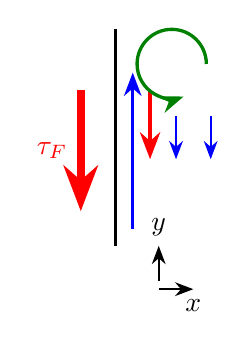
\begin{tikzpicture}[scale=1.1, >=Stealth]

    % draw the sidewall going up/down:

    \draw[very thick] (0,0) -- (0,2.5) node[midway, right] {};
    % draw a blue arrow pointing north to the left of the sidewall:
    \draw[->, very thick, blue] (0.2,0.2) -- (0.2,2.);
    % draw a couple of small arrows going south to the left of this big arrow:
    \draw[->, thick, blue] (0.7,1.5) -- (0.7,1.0);
    \draw[->, thick, blue] (1.1,1.5) -- (1.1,1.0);

    % draw a very very thick red arrow pointing north to the right of the sidewall and label $\tau_F(x)$:
    \draw[->, very thick, red, line width=3] (-0.4,1.8) -- (-0.4,0.4) node[midway, left] {$\tau_{F}$};
    \draw[->, very thick, red, line width=1.5] (0.4,1.8) -- (0.4,1.0) node[midway, right] {};

    % draw a circle with an arrow indicating clockwise rotation:
    \draw[->, very thick, darkgreen] (1.05,2.1) arc[start angle=0, end angle=290, radius=0.4] node[midway, right] {};

    % small axes indicating x and y directions:
    \draw[->, thick] (0.5, -0.5) -- (0.9, -0.5) node[below] {$x$};
    \draw[->, thick] (0.5, -0.40) -- (0.5, 0.0) node[above] {$y$};


\end{tikzpicture}
\end{document}
